\chapter{Atividades realizadas}
\label{ch:3}

\section{Modelagem}
\label{sec:mod}

O projeto DataUSP-PosGrad iniciou-se na Pró-reitoria de Pós-graduação da Universidade de São Paulo (USP) em 2012, com a modelagem dos dados para a criação de um Data Warehouse. Com o domínio dos dados bem definido, iniciou-se o processo de modelagem do sistema e a escolha das tecnologias que seriam utilizadas em sua construção. O Departamento de Tecnologia da Informação da USP, que é a equipe responsável por fazer a manutenção e desenvolver novos sistemas para a universidade, utiliza por padrão a linguagem de programação Java juntamente com o sistema gerenciador de banco de dados Sybase ASE. 
\par
Deste modo os requisitos básicos do sistema foram definidos como:

\begin{enumerate}

\item Linguagem de programação Java;
\item Interface web para interação com o usuário;
\item Orientado a serviços (Serviço Web);
\item Banco de dados Sybase ASE;

\end{enumerate}

Por ser orientado a serviços o sistema foi então dividido em duas grandes componentes: O servidor de recursos e uma interface web(aplicação cliente) para a exibição dos dados.

\subsection{Servidor de recursos}
\label{sub:server}

Um Serviço Web pode interagir com outros serviços e não exclusivamente com uma única aplicação. Portanto ele deve dispor de um mecanismo de requisição de seus recursos, ou seja, uma interface de acesso. Para facilitar a escalabilidade e a manutenção do sistema foi decidido então que o DataUSP-PosGrad seria implementado seguindo as premissas do REST~\ref{sec:rest} por meio do framework Jersey~\ref{sec:jersey}. Além disso, o formato de dados JSON (JavaScript Object Notation) foi adotado como padrão para a troca de mensagens. 
\par
O JSON é um formato texto para a troca de dados completamente independente de linguagem. Utiliza convenções que são familiares às linguagens C , C++, C\#, Java, JavaScript, Perl, Python dentre outras. É uma estrutura de dados simples, leve e fácil de ser interpretada por humanos e também por computadores. Sua estrutura é composta por um conjunto de pares chave e valor do com a seguinte sintaxe: {chave1 : valor1, chave2 : valor2, … }. As chaves são cadeias de caracteres e os valores podem ser diversos tipos de objetos, dependendo da linguagem utilizada, como listas, dicionários, números, ou até mesmo outros JSON.
\par
Como uma interface web será o principal consumidor dos recursos do servidor, o formato JSON é adequado para a comunicação, uma vez que quem a executa é um navegador de internet. Os navegadores de internet, também conhecidos por Web Browsers (por exemplo o Mozilla Firefox, Google Chrome, Internet Explorer e etc), têm motores específicos para executar código JavaScript e por conseguinte interpretam o formato JSON nativamente.

\subsection{Interface Web}
\label{sub:inter}

A Interface Web é um cliente que utiliza os Serviços Web no DataUSP-PósGrad. Sua função é requisitar os dados ao servidor de recursos, de acordo com os parâmetros fornecidos pelo usuário do sistema,e construir relatórios Ad-Hoc (relatórios sob demanda), por meio de gráficos e tabelas. Além disso a Interface Web deve ser capaz de receber e enviar arquivos ao servidor, como também enviar informações de autenticação do usuário. Desse modo, a seguinte lista de requisitos deve ser atendida em sua implementação:

\begin{enumerate}

\item Integração com o login único da USP de autenticação;
\item Exibição de gráficos em três dimensões interativos e renderizados em tempo real;
\item Utilizar a biblioteca JQuery~\ref{sub:jq} para a manipulação dos dados;
\item 4. Interagir com o servidor de recursos por meio de requisições assíncronas AJAX~\ref{sub:aj}.

\end{enumerate}

A biblioteca FusionCharts~\ref{sub:fc}, utilizada para renderização gráfica, foi escolhida por atender os requisitos do sistema e por sua diversidade de modelos de gráficos. Nessa etapa de modelagem da Interface Web também foram definidos seu leiaute, cores e padrões de desenho.

\subsection{Consultas}

Definida a arquitetura do sistema, iniciou-se o processo de modelagem dos relatórios analíticos, que são basicamente as consultas SQL~\ref{sec:sql} responsáveis por buscar os dados no DataWarehouse.  Além das consultas para gerar relatórios foram definidas ainda as consultas de controle e as consultas de filtragem. 
\par
As consultas de controle buscam dados relativos às permissões de acesso dos usuários, como a unidade a que pertencem, a quais programas e áreas ele tem acesso e quais os relatórios que eles podem gerar. Já as consultas de filtragem permitem que o usuário selecione dados específicos dentro de seu escopo de visualização, filtrando as informações mostradas nos relatórios.

\subsection{Usuários}
Os usuários foram classificados em grupos de acordo com a permissão de acesso dentro do sistema. São eles:
\begin{itemize}
\item \emph{Nível 1} - Grupo responsável pelo sistema, não tem restrição de acesso (usado apenas para desenvolvimento);
\item \emph{Nível 2} - É o nível máximo que tem permissão total de acesso (Reitor e vices, Pró-reitor de pós-graduação);
\item \emph{Nível 3} - Usuário comum que tem permissão apenas aos seus programas e áreas específicos (Coordenadores e presidentes de CCP e CPG, assim como seus suplentes);
\end{itemize}

\section{Construção do sistema}

Uma vez determinadas as tecnologias a serem utilizadas, iniciou-se o processo de construção de um arcabouço, afim de testar as funcionalidades de Serviços Web do Jersey~\ref{sec:jersey}. Os detalhes técnicos e arquiteturais da linguagem Java apresentados nesta seção, encontram-se na seção~\ref{sec:java}. 
\par
Esse esqueleto do DataUSP-PósGrad tem a seguinte estrutura:

\begin{figure}[H]
    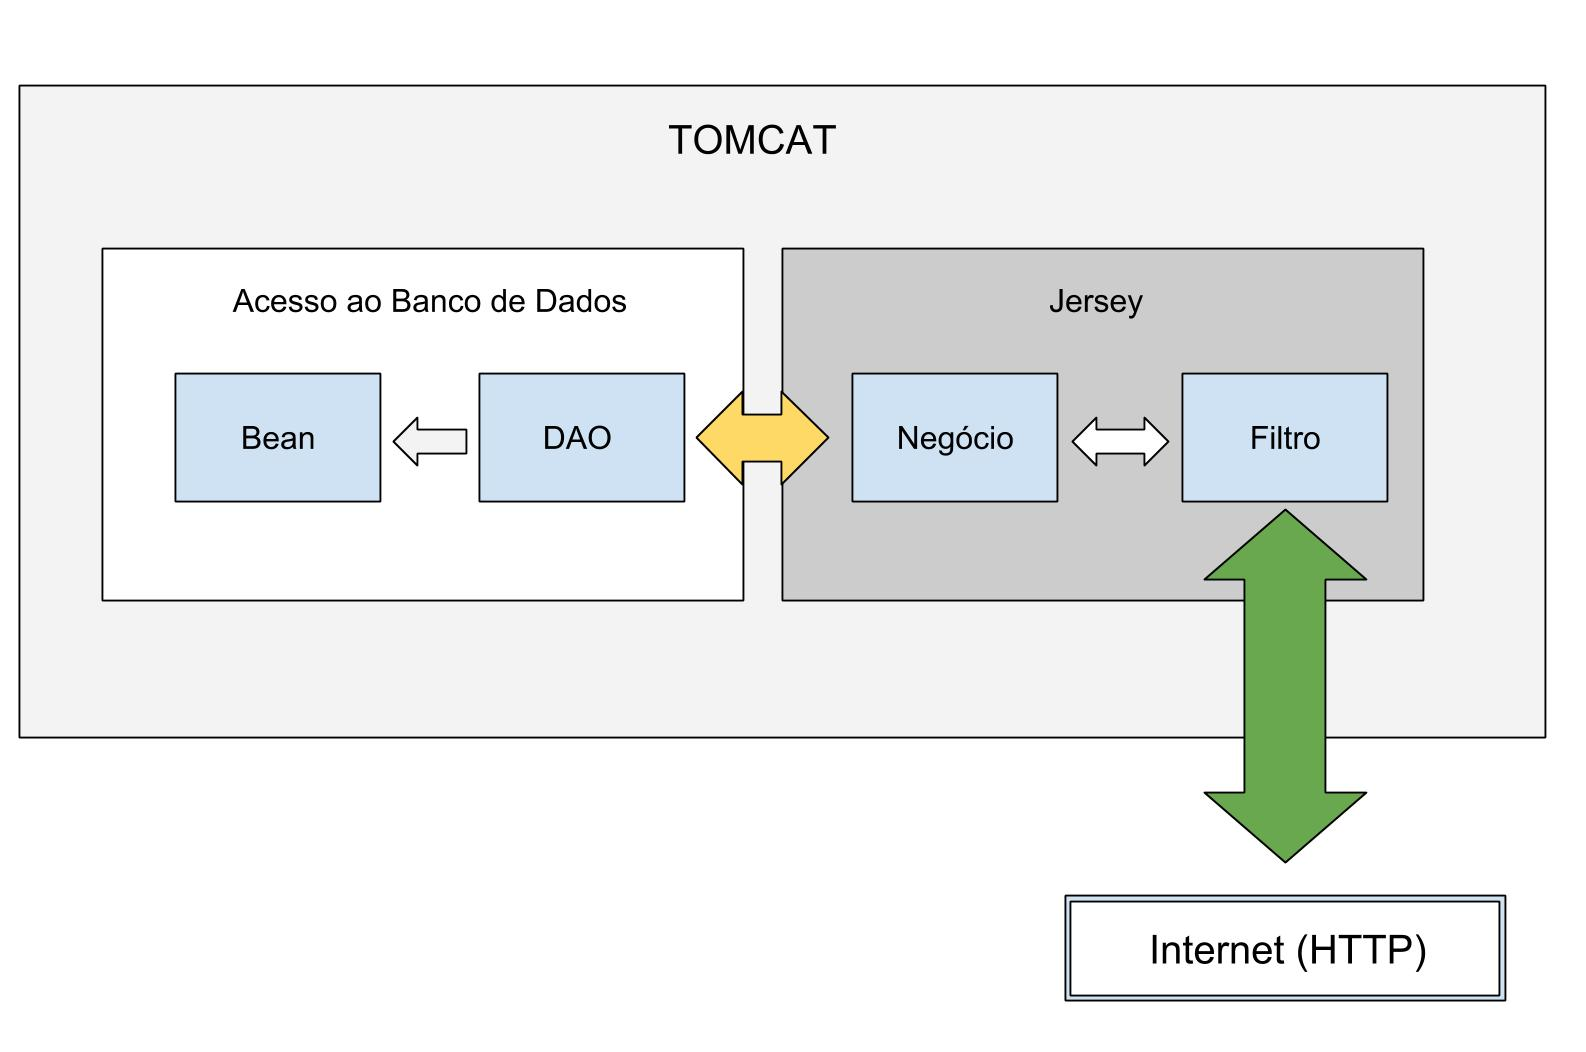
\includegraphics[width=\textwidth]{figuras/skel}
    \caption{Esqueleto do DataUSP-PósGrad}
    \label{fig:skel}
\end{figure} 

\begin{enumerate}
\item \textbf{Tomcat}O servidor Apache Tomcat é um contêiner Web de código aberto. Foi desenvolvido para executar aplicações Web que utilizam as tecnologias Java Servlet e JavaServer Pages. Ele é responsável por instanciar as classes Java de acordo com as requisições web recebidas;

\item \textbf{Filtro} - Todas as requisições atendidas pelo Tomcat seguem por um filtro do Jersey, responsável por validar e autenticar o acesso a todos os recursos disponíveis no Web Service;

\item \textbf{Negócio} - Classe de negócio contém a lógica responsável por tratar as requisições. Os métodos públicos dessa classe são a implementação dos recursos do Serviço Web (que é a própria classe Java). Cada um desses métodos públicos é identificado por meio de anotações, que nada mais são do que o identificador único de cada recurso, ou seja, seu endereço na rede;

\item \textbf{Data Access Object (DAO)} -  Classe Java responsável por abstrair a interação das classes de negócio com o banco de dados. O DAO gerencia a conexão, executa as consultas SQL ou procedimentos armazenados na base de dados (Stored Procedures) e, retorna os dados à classe de negócio;

\item \textbf{Bean} - Essa classe encapsula os atributos que representam as colunas de uma tabela no banco de dados. É usada pelo DAO para retornar o resultado de uma consulta.
\end{enumerate}

\subsection{Funcionamento}
\label{sub:func}
Ao receber uma requisição por um recurso, o Tomcat instancia o filtro e a classe Java de Negócio referente ao Serviço Web solicitado. Isso é feito utilizando-se o endereço único de tal recurso por meio das Anotações em Java.  
\par
O Filtro então autentica o usuário do serviço e transfere a solicitação para o Negócio que, por sua vez, executa seu método público referente ao recurso requisitado (novamente por meio do uso de anotações em Java). Os métodos públicos (recursos) das classes de Negócio (Serviços Web), contém ainda outras anotações referentes ao método HTTP de acesso(@GET, @POST, etc) e também aos formatos de dados recebidos(@Consumes) e enviados (@Produces). 
\par
O método público correspondente ao recurso solicitado instancia um DAO, que busca os dados no banco e os retorna uma lista de BEAN. Cada BEAN nessa lista corresponde a uma linha da tabela gerada pela consulta sql executada no banco.  Esses dados então são processados para gerar a resposta enviada ao usuário do recurso, por meio do protocolo HTTP.

\subsection{Exemplo de funcionamento}
\label{sub:exemplo}

Por meio da Interface Web, um usuário do DataUSP-PósGrad pode, por exemplo, gerar um relatório
com a quantidade de titulações do programa de Ciência da Computação do Instituto
de Matemática e Estatística, em um intervalo de anos:

\begin{itemize}
\item{O cliente (Interface Web) solicita o recurso "número de títulos" por meio do seguinte endereço:} \hfill 
\\[2ex]
\scriptsize{http://uspdigital.usp.br/datausppg/servicos/relatorio/numero\_titulos/45/45005/45134/1998/2013}
\\[4ex]
\normalsize Note que após \dots numero\_titulos/ os números significam:
    \begin{itemize}
        \item 45 -> Código da unidade;
        \item 45005 -> Código do programa;
        \item 45134 -> Código da área;
        \item 1998 -> Ano inicial;
        \item 2013 -> Ano final.
    \end{itemize}
 \item{O servidor atende a requisição~\ref{sub:func} e retorna os dados no formato json~\ref{sub:server}:} \hfill 
\\[3ex]
\scriptsize{\{"anoInicial":1998,"anoFinal":2013,\\
"totalME":[0,4,11,20,20,23,28,24,25,32,34,17,26,38,43,22],\\
"totalDO":[0,0,3,2,1,3,5,2,3,4,5,3,6,6,13,5],\\
"totalDD":[0,0,0,0,1,0,0,0,0,1,1,0,1,1,1,0],\\
"totalDODD":[0,0,3,2,2,3,5,2,3,5,6,3,7,7,14,5],\\
"totalGeral":[0,4,14,22,22,26,33,26,28,37,40,20,33,45,57,27]\}}
\\[6ex]
\normalsize Esse json contem quatro listas referentes à quantidade de títulos nos cursos de Mestrado (totalME),
 Doutorado (totalDO), Doutorado Direto (totalDD) e a soma das três anteriores (totalGeral), no intervalo de "anoInicial" a "anoFinal".
\end{itemize}
A Interface Web então constrói o relatório e exibe os dados ao usuário como na figura~\ref{fig:tit}. 
\begin{figure}[H]\centering
  \caption{Interface Web do DataUSP-PósGrad}\label{fig:tit}
  \centerline{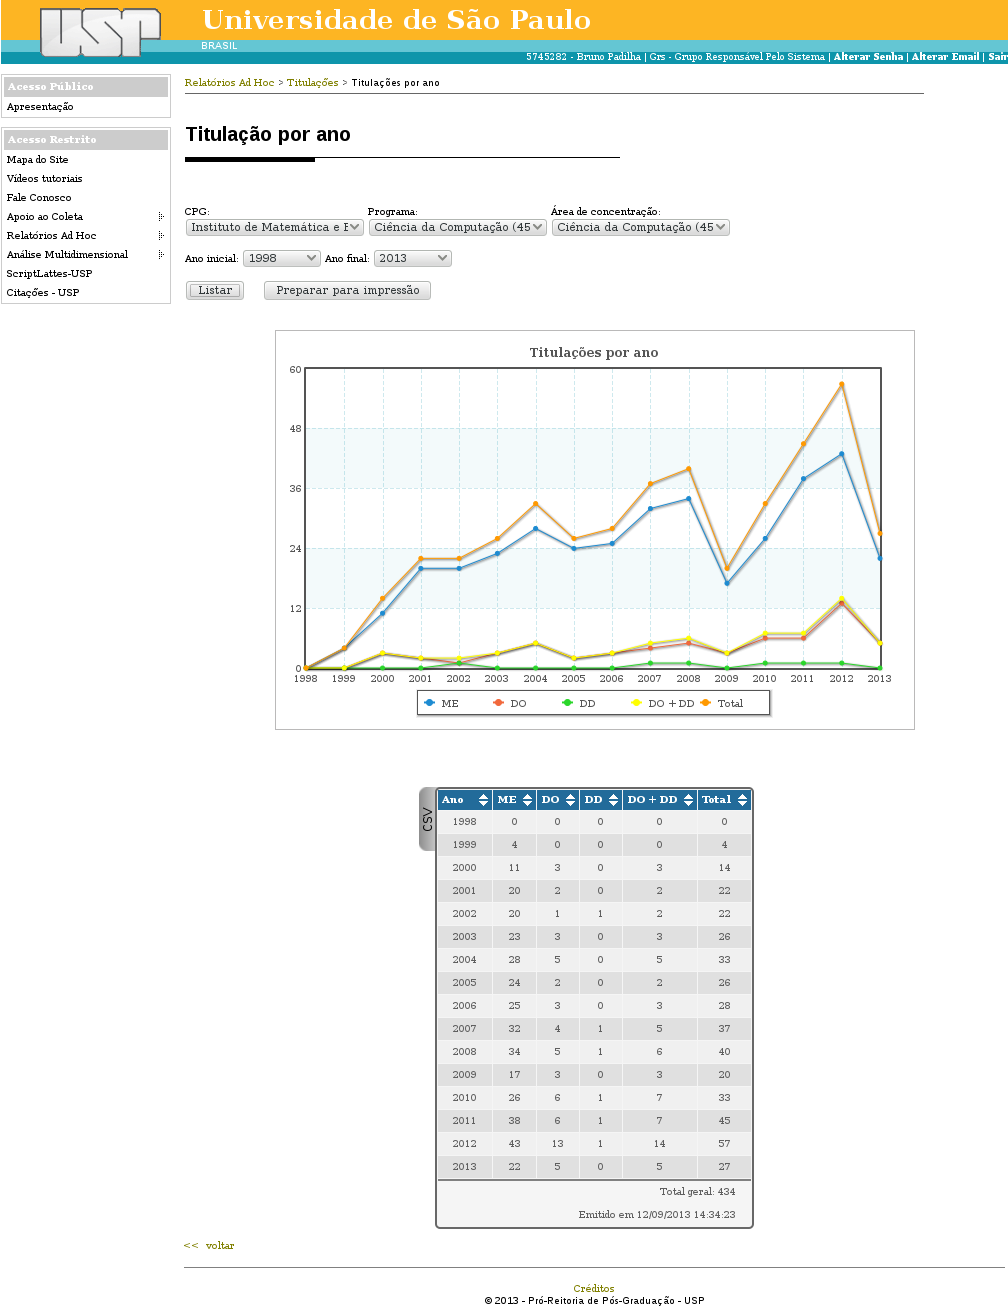
\includegraphics[width=\textwidth]{figuras/telatitulo.png}}
\end{figure}

\section{Relatórios Ad-hoc}

Os relatórios Ad-hoc são gerados dinamicamente e, em geral, exibem os dados na forma de um gráfico interativo e também em uma tabela, que pode ser exportada como uma planilha. São classificados em quatro grupos principais conforme o interesse da Universidade:

\begin{enumerate}
\item \textbf{Titulações} - Estatísticas quantitativas dos docentes, programas e áreas da pós-graduação;
\item \textbf{Egressos} - Situação dos alunos egressos;
\item \textbf{Internacionalização} - Estrangeiros em cursos de pós-graduação da USP;
\item \textbf{Produção Coleta} - Produção intelectual dos orientadores e orientandos.
\end{enumerate}

\subsection{Titulações}
\subsubsection{Titulações por ano}
\label{subsub:titano}
Esse relatório exibe a quantidade de títulos de mestrado, doutorado e doutorado direto para cada área
da pós-graduação na USP, desde o ano de 1970. Foi o primeiro relatório do DataUSP-PósGrad, serviu para consolidar o modelo~\ref{sec:mod}, fazer alguns ajustes no Data Warehouse e explorar as funcionalidades do Fusion Charts~\ref{sub:fc}(animações, tipos de gráficos, cores e etc). Veja a figura~\ref{fig:tit}  

\subsubsection{Tempo médio de titulação por programa}
Exibe o tempo médio para se obter um título de mestrado, doutorado e doutorado direto em meses. Pode-se mostrar todas as áreas de um dado programa no mesmo gráfico.

\subsubsection{Tempo médio de titulação por docente}
\label{ssc:td}
Exibe o tempo médio em meses de titulação dos orientandos por docente. Ao escolher uma área será exibida uma lista com todos os orientadores cadastrados, onde pode-se selecionar um ou mais para exibir os dados em um mesmo gráfico.

\subsubsection{Teses por programa}
Numero total de teses dividido pelo numero de docentes de uma área.

\subsubsection{Teses por docente}
Do mesmo modo que em~\ref{ssc:td}, um lista de docentes é exibida mas será gerado um gráfico para cada um dos selecionados, com o seu número de teses de mestrado, doutorado e doutorado direto no intervalo escolhido.

\subsubsection{Downloads de teses por docente}
Mostra uma lista com a quantidade de downloads da produção intelectual dos docentes na Biblioteca Digital de Teses e Dissertações~\footnote{BDTD - \texttt{http://bdtd.ibict.br/}}. Atualmente esta funcionalidade está desativada por um erro de inconsistência nos dados informados pela BDTD.

\subsection{Egressos}
Após conseguir um título de pós-graduação, os alunos egressos podem responder um questionário que tem por objetivo traçar um perfil de sua atuação profissional. Com a devida validação desses dados é possível saber, por exemplo a quantidade de egressos que atuam em empresas privadas, em cargos públicos, na área acadêmica e etc.
\par Alguns relatório de egressos foram desativados, até que se possa validar os dados dos questionários de modo mais rigoroso, para evitar erros e inconsistências. 

\subsubsection{Distribuição de respostas por colegiado}
Calcula a quantidade de questionários respondidos por cada unidade da USP.

\subsubsection{Total de respostas por conclusões}
Como no relatório anterior porém relativamente ao numero total de egressos por unidade.

\subsection{Internacionalização}

\subsubsection{Alunos por País}
Exibe a distribuição dos alunos estrangeiros por país em cursos de pós-graduação na USP.

\subsubsection{Estrangeiros em estágio de média/longa duração}
Alunos estrangeiros em cursos de pós-graduação na USP que estão realizando estágio com mais de 3 meses de duração.

\subsubsection{Estrangeiros em estágio de curta duração}
Como no relatório anterior porém para estágio com menos de 3 meses de duração.

\subsubsection{Alunos de duplo diploma}
Alunos brasileiros ou estrangeiros que fizeram parte do curso na USP e parte em universidade estrangeira, obtendo dois diplomas.

\subsection{Produção Coleta}
São relatórios da produção intelectual da pós-graduação, de acordo com os dados que são enviados anualmente à Capes para análise.

\subsubsection{Produção por Estrato}
\label{sub:pes}
Relatório com a classificação Qualis\footnote{Avaliação Qualis - \texttt{http://www.capes.gov.br/avaliacao/qualis}} da
produção dos programas de pós-graduação. Veja a figura~\ref{fig:qualis}

\begin{figure}[H]
    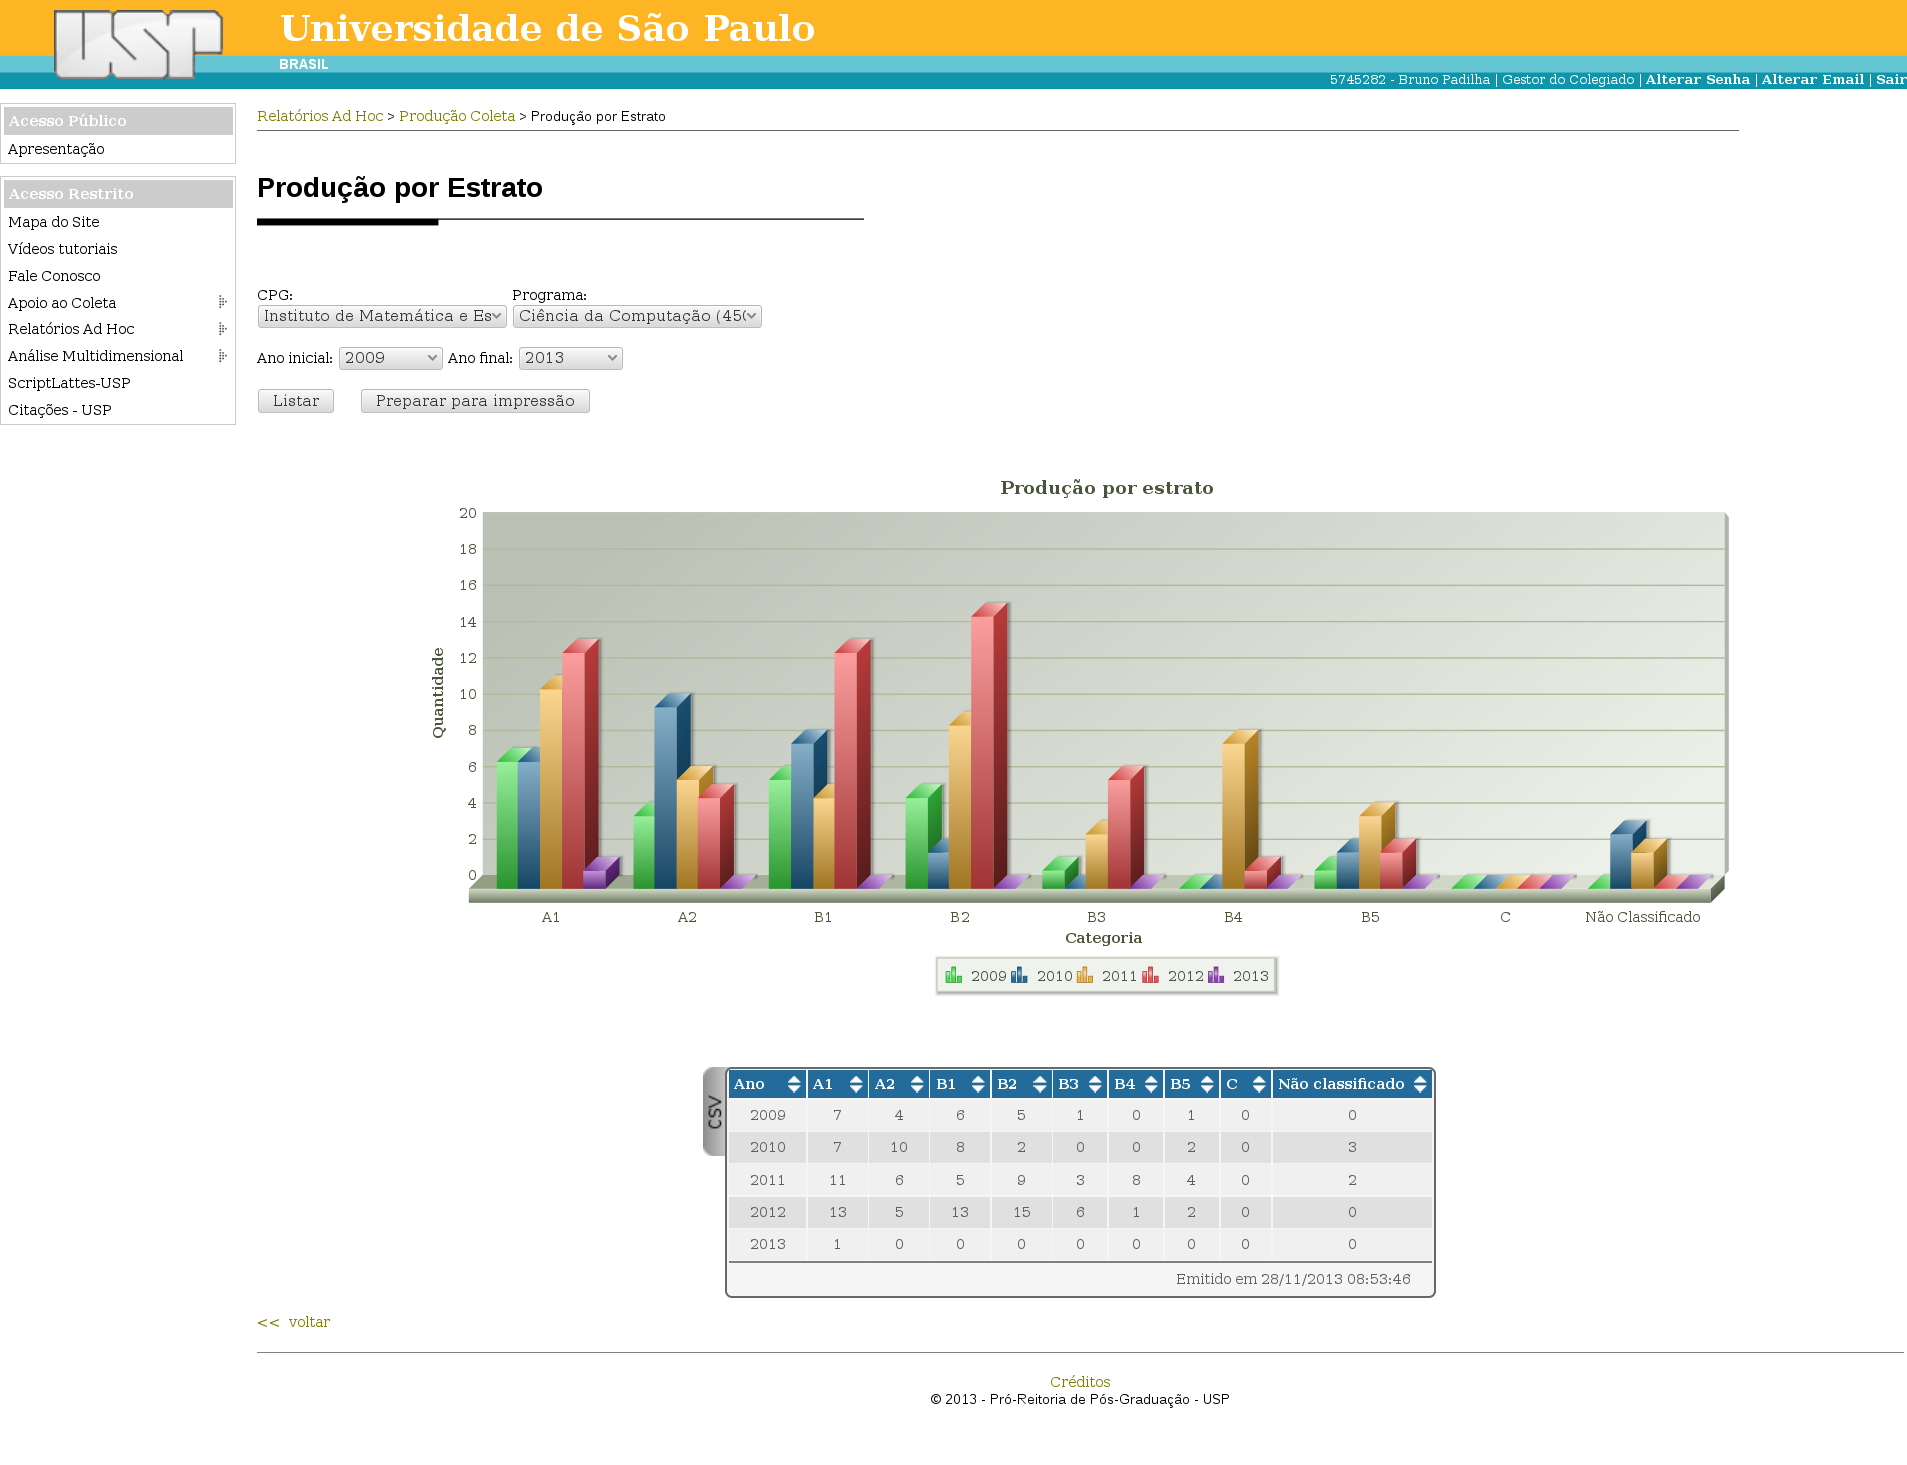
\includegraphics[width=\textwidth]{figuras/qualis.png}
    \caption{Produção intelectual por extrato}
    \label{fig:qualis}
\end{figure}
\vfill
\subsubsection{Produção Total}
\label{sub:ptot}
Classificação do tipo de produção por programa em um dado intervalo de tempo. Alguns exemplos:
\begin{itemize}
\item Apresentação de trabalho;
\item Artigo em jornal ou revista;
\item Artigo em periódico;
\item Livro
\item Trabalho em anais
\end{itemize}

\section{Análise Multidimensional}
\label{sec:amult}
Principalmente por se tratar de um sistema analítico, o DataUSP-PosGrad é intrinsecamente orientado a dados. Uma estrutura multidimensional de dados, o cubo MOLAP~\ref{sub:multi}, é essencial para a flexibilidade e eficiência das consultas que, basicamente, navegam no cubo em busca de uma informação específica.
\par
Para ampliar a cobertura dos relatórios Ad-hoc e também para permitir que cada unidade da USP possa gerar suas próprias análises, o DataUSP-PosGrad fornece acesso direto ao cubo MOLAP, segmentado por unidade da USP, por meio de um visualizador chamado Saiku\footnote{Saiku - http://meteorite.bi/saiku}. No Saiku o usuário pode selecionar as dimensões do cubo pertinentes e filtrar os resultados para obter os dados em forma de uma tabela. Veja um exemplo na figura~\ref{fig:saiku}

\begin{figure}[H]
    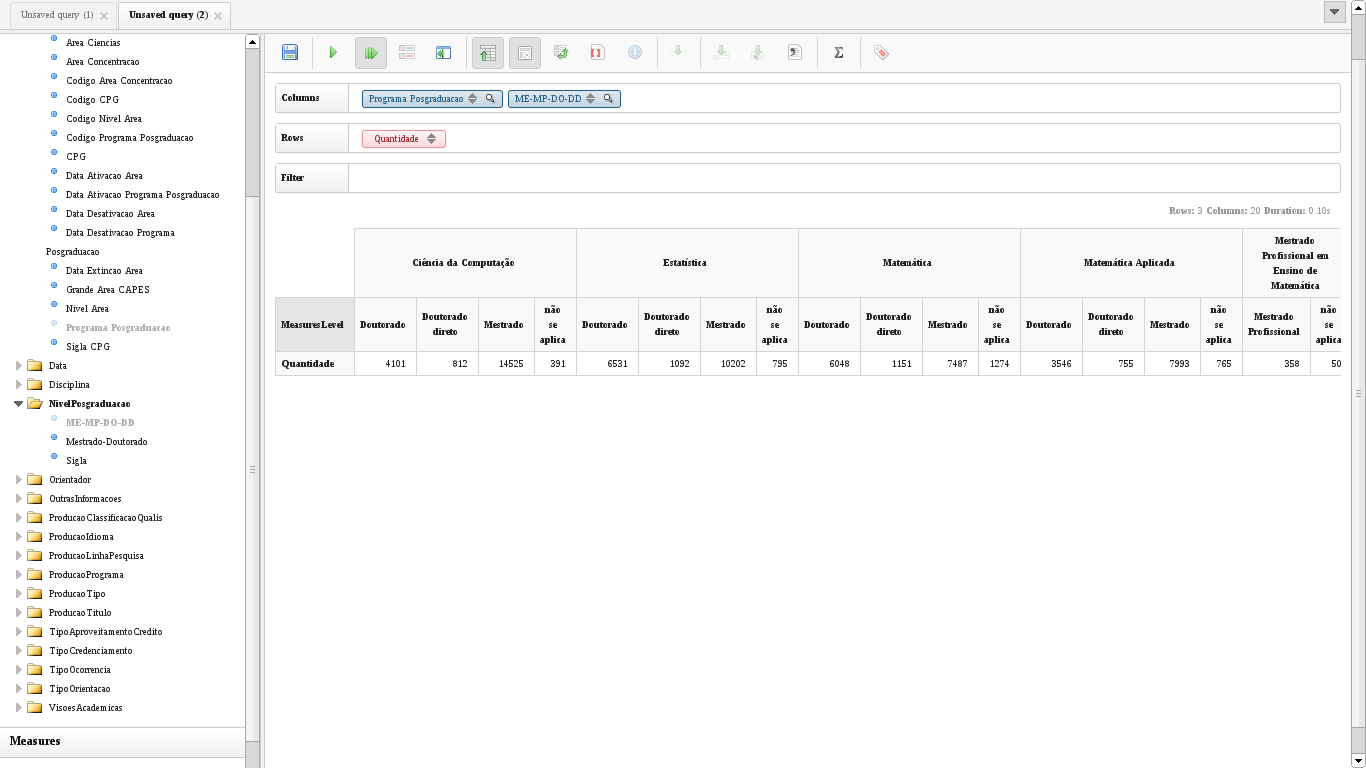
\includegraphics[width=\textwidth]{figuras/saiku.png}
    \caption{Exemplo de consulta dinâmica no cubo MOLAP usando o visualizador Saiku}
    \label{fig:saiku}
\end{figure}
 
Cada usuário pode baixar uma versão \emph{offline} do cubo MOLAP da unidade USP a qual esteja vinculado, que pode ser visualizado com o Microsoft Excel.
\par
Um exemplo da versatilidade de um Serviço Web RESTful é o recurso de download de arquivos no DataUSP-PósGrad. Uma solicitação de download responde com o próprio arquivo e não com o caminho onde o mesmo se encontra, ou seja, o formato de dados da resposta do recurso de download são os bytes conjuntamente com as metainformações de tamanho, nome e tipo do arquivo. Isso é feito modificando-se o cabeçalho da requisição por meio do protocolo HTTP, que já é usado como interface de acesso ao serviço. Quem solicita esse recurso tem então a capacidade de reconstruir o arquivo.
\par
Essa alternativa de controle de download aumenta a segurança de acesso aos arquivos, uma vez que o caminho onde os mesmos
se encontram no servidor nunca é revelado a quem consome tal recurso.

\section{Citações-USP}
\label{sec:cita}
Ao publicar um artigo, periódico, livro ou algum outro trabalho científico, o autor geralmente acaba citando outros trabalhos utilizados em sua pesquisa. O impacto da produção de um autor em uma dada literatura pode ser medida por meio da quantidade de citações de seus trabalhos.
\par A quantidade de publicações e de suas respectivas citações definem uma métrica quantitativa denominada \emph{índice-h}~\cite{h-index}. O índice-h é calculado como o número \emph{ncit} de publicações de um autor que tenham ao menos \emph{ncit} citações cada.
\par As principais fontes que contabilizam o número de citações são o \emph{Google Scholar}\footnote{Google Acadêmico - \texttt{http://scholar.google.com.br/}}, o \emph{Scopus}\footnote{Scopus - \texttt{http://www.elsevier.com/online-tools/scopus}} e o \emph{Web of Science}. O DataUSP-PósGrad, por meio da técnica de \emph{Web Crawling}~\ref{sec:wc}, varre o Google Scholar e também o Scopus em busca de dados de publicações dos docentes da USP. Futuramente serão inclusos também os dados do Web of Science.
\par
A figura~\ref{fig:cit} ilustra um exemplo de visualização dos dados de citações.

\begin{figure}[H]
    \centering 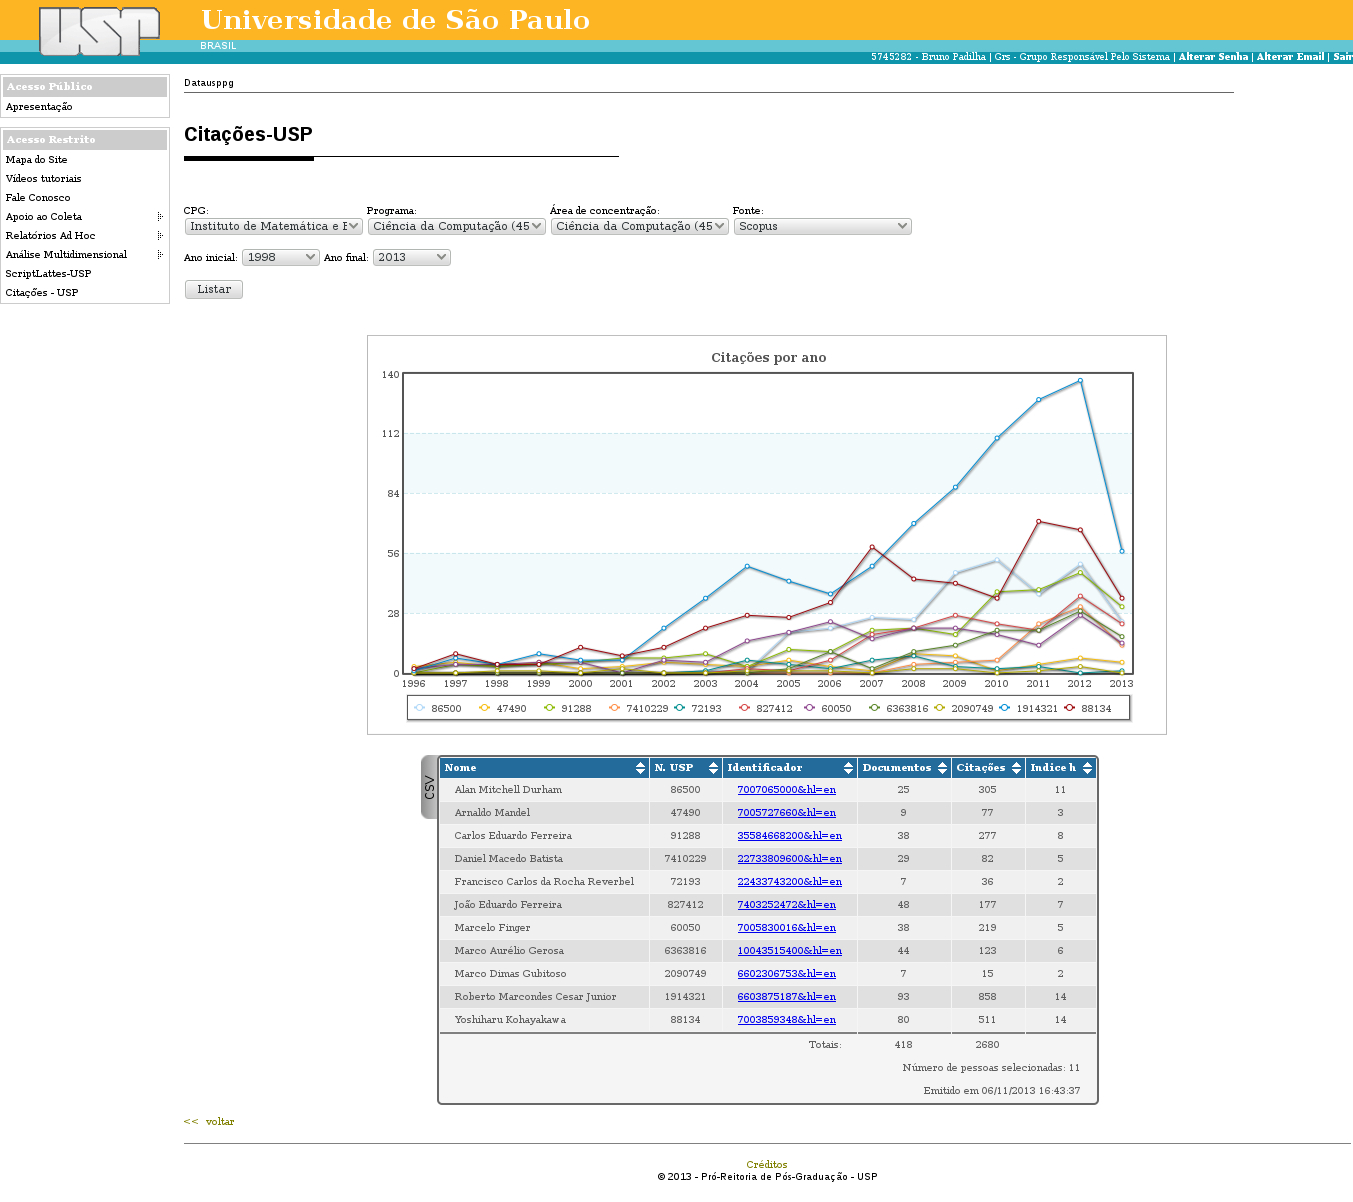
\includegraphics[width=0.8\textwidth]{figuras/dtausp_citacoes}
    \caption{Gráfico comparativo com o número de citações de alguns docentes do IME}
    \label{fig:cit}
\end{figure} 

\subsection{Funcionamento do Web Crawler}

Como essa parte do sistema foi escrita em Python, a interface com os bancos de dados (leitura e escrita) é feita
por meio da ferramenta Kettle do Pentaho~\ref{sec:pentaho}, já que não foi possível fazer com que o Web Crawler interagisse
diretamente com os bancos de dados Sybase ASE, utilizados na USP.
\par
Inicialmente, um script Kettle busca os dados dos docentes no banco (nome, número usp, programa a que pertence, etc) e gera um arquivo com essas informações. O Web Crawler então processa esse arquivo de entrada e, para cada docente, varre as páginas do Google Scholar e também do Scopus em busca dos dados de citações. Os dados gerados pelo Web Crawler são armazenados em um outro arquivo que, finalmente, é processado por um outro script Kettle que os insere no banco de dados.
\par
Cada docente cadastrado no Google Scholar ou no Scopus possui um respectivo identificador único. Como a principio esses identificadores não estão armazenados nos bancos de dados da USP, a primeira tarefa do Web Crawler é fazer a associação desses identificadores aos docentes. A busca pelos identificadores é feita pelo nome do docente, considerando alguns outros parâmetros de similaridade como o nome da universidade, instituto e endereço de email. Ainda assim o nome do docente cadastrado na USP pode não ser exatamente igual ao buscado nas páginas, portanto o casamento de padrão no nome é feito heuristicamente.
\par
O passo anterior apenas é executado para docentes que ainda não possuem seus identificadores Scopus ou Scholar associados ao seu número usp. O processo de atualização é similar, porém a busca é feita diretamente pelo identificador, o que torna o processo consideravelmente mais ágil e preciso.
\par
Por se tratar de um processo heurístico, nem sempre os números usp e identificadores são associados corretamente. Para suprir essa deficiência, na Interface Web do DataUSP-PósGrad, o usuário tem a opção de corrigir um identificador, ou ainda informar um outro que não tenha sido encontrado pelo Web Crawler. Assim a tendência é que os dados se consolidem pelos próprios usuários.

\newpage

\section{Outros Serviços}
Dois outros sistemas já existentes foram incorporados ao DataUSP-PósGrad: o \emph{ScriptLattes}~\cite{sclt}, no formato de uma ferramenta ; um outro sistema administrativo da pró-reitoria de pós-graduação da USP, anteriormente conhecido por Gerência-Pós, em forma de serviços.

\subsection{ScriptLattes}
O ScriptLattes é uma ferramenta para fazer análises de dados obtidos da plataforma \emph{Lattes}\footnote{CNPQ Lattes - \texttt{http://lattes.cnpq.br/}}. Foi desenvolvido em Python e utiliza um arquivo de configuração onde, por meio do identificador lattes~\footnote{O identificador lattes é um número como \emph{"0131770792108992"} que identifica unicamente um pesquisador cadastrado na plataforma}, são descritos os autores dos quais se deseja baixar os currículos.

\begin{figure}[H]
\begin{minted}[frame=single,linenos,mathescape,fontsize=\scriptsize,label=exemplo.list]{py3}
# Lista de professores (linhas de comentarios comecam com '#')
4575931307749163,Carlos Hitoshi Morimoto, 1999-HOJE, Professor
0131770792108992,Joao Eduardo Ferreira, 1999-2006 & 2006-HOJE, Professor
0362417828475021,Junior Barrera, 1992-2008, Professor
0926213060635986,Marcel Parolin Jackowski, 2006-HOJE, Professor
0644408634493034,Nina Sumiko Tomita Hirata,,Professor # membro sem periodo
1647118503085126,Roberto Hirata Junior,, Professor # membro sem periodo
2240951178648368,Roberto Marcondes Cesar Junior, 1998-HOJE, Professor
9283304583756076,Ronaldo Fumio Hashimoto,, Professor # membro sem periodo

# lista de colaboradores
4727357182510680,Jesus P. Mena-Chalco, 1995-1999 & 2005-HOJE, Colaborador

# lista de alunos
2837012019824386,Andrea Britto Mattos,, Aluno# membro sem periodo
\end{minted}
\caption{Arquivo de configuração do ScriptLattes que contém a lista de pesquisadores}
\label{lst:slattes}
\end{figure}

Um outro arquivo de configuração com os parâmetros da análise, contendo o caminho dos arquivos (por exemplo o caminho do arquivo~\ref{lst:slattes} e configurações gerais do script, também é necessário. 
\par
Além de o usuário precisar conhecer previamente os identificadores lattes das pessoas em análise, requer-se um certo conhecimento sobre o ambiente onde o ScriptLattes será executado (instalar dependências, configurar permissões, criar os arquivos de configuração do script e etc).
\par 
Com o propósito de potencializar seu uso, o ScriptLattes foi integrado ao DataUSP-PósGrad. Na Interface Web, uma lista de pesquisadores é exibida (no formato dos relatórios ad-hoc~\ref{fig:tit}) onde o usuário seleciona um grupo, inclusive filtrando por unidade ou área. Em seguida são gerados os arquivos de configuração automaticamente e o ScriptLattes
é executado no Servidor de Recursos~\ref{sub:server}, e o resultado da análise é exibido na Interface Web.
\par 
Essa abstração da execução do ScriptLattes facilita o uso da ferramenta para os usuários do DataUSP-PósGrad, que tem ainda a possibilidade de receber os resultados da análise por email.
\par
A figura~\ref{fig:ldta} ilustra o resultado de uma análise realizada pelo ScriptLattes dentro do DataUSP-PósGrad.
\begin{figure}[H]
    \centering 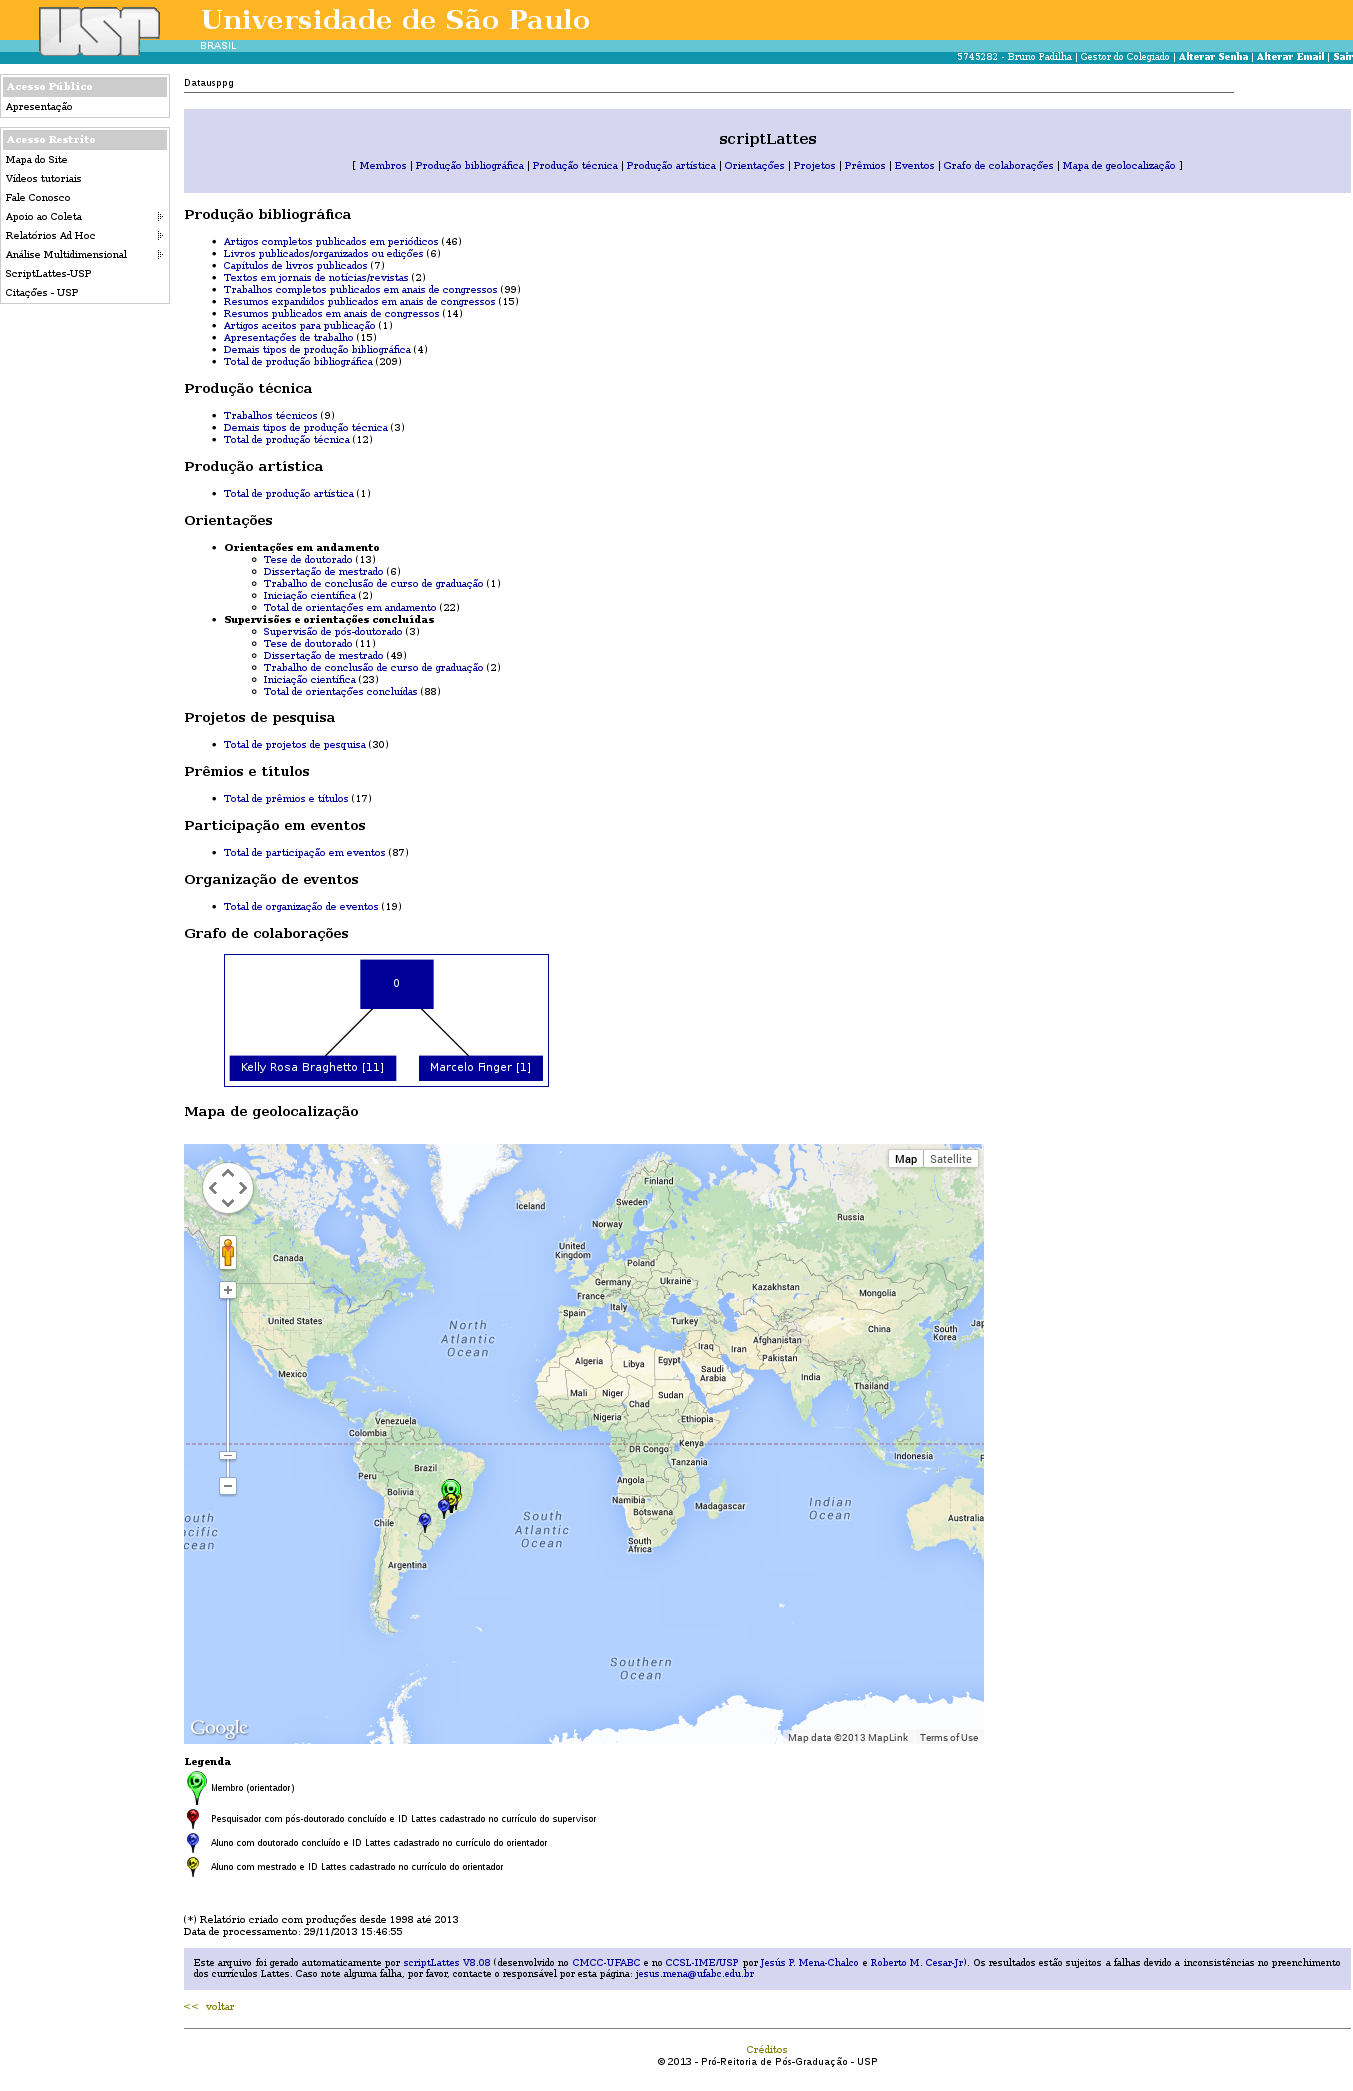
\includegraphics[width=0.9\textwidth]{figuras/lattes.png}
    \caption{ScriptLattes dentro do DataUSP-PósGrad}
    \label{fig:ldta}
\end{figure}
\vfill

\subsection{Gerência-Pós (Apoio ao coleta)}
\label{sub:coleta}
O Gerência-Pós é um conjunto de ferramentas para extração e análise dos dados enviados à Capes anualmente para a avaliação dos programas de pós-graduação. Agiliza o processo de coleta dos dados automatizando o preenchimento de formulários, além de gerar um relatório histórico do \emph{extrato WebQualis}.
\par Sua principais ferramentas foram transformadas em serviços e incorporadas ao DataUSP-PósGrad (por exemplo os relatórios~\ref{sub:pes} e~\ref{sub:ptot}) com o nome de \emph{Apoio ao Coleta}. 
\par No menu do apoio ao coleta, dentro do DataUSP-PósGrad, é possível enviar o arquivo no formato coleta capes de um programa para fazer a análise em tempo real. Isso é feito de modo similar ao download dos cubos offline~\ref{sec:amult}, mas agora há um recurso no servidor que recebe o arquivo em formato binário. Por parte da interface web o envio de arquivos é feito de maneira assíncrona via Ajax~\ref{sub:aj} e HTML5~\ref{sub:h5}, e o resultado da análise é retornado em seguida\footnote{O uso de HTML5 é necessário para extrair o conteúdo binário do arquivo selecionado em um formulário, e também para exibir o progresso do upload ao usuário, a exemplo do que é utilizado no Gmail, o serviço de emails do Google, para envio de arquivos anexos}.
\par Outra funcionalidade disponível no mesmo menu é fazer a análise anterior automaticamente, porém para o triênio (últimos 3 anos, figura~\ref{fig:trim}) e sem a necessidade de envio de arquivos.

\begin{figure}[H]
    \centering 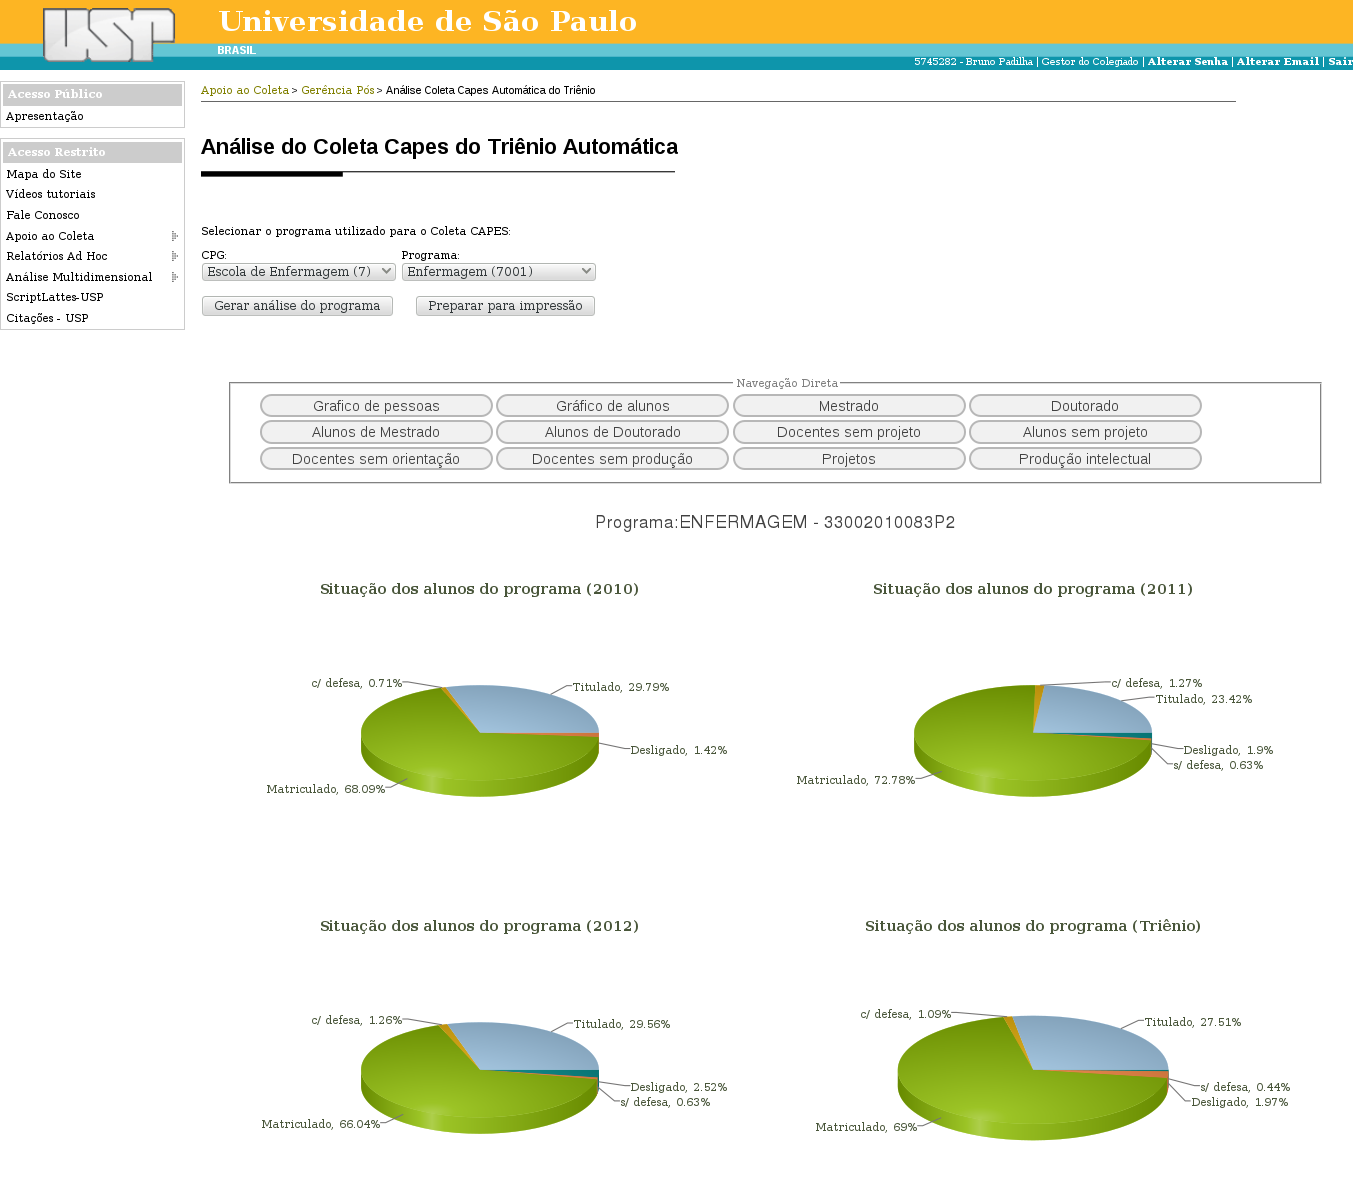
\includegraphics[width=0.5\textwidth]{figuras/trienio.png}
    \caption{Imagem parcial do relatório de análise do triênio}
    \label{fig:trim}
\end{figure} 

